O último filtro deste trabalho é o de nitidez, também chamado de \textit{sharpen} ou agudização. No espaço das frequências, esse tipo de filtro é responsável por enfraquecer frequências mais baixas, por isso é chamado de filtro passa-altas. Isso faz com que esse filtro seja um tipo de processo "inverso"\ do filtro de \textit{blur} (\cref{sec:blur}).

Assim como os filtros de \textit{blur}, filtros de nitidez têm a soma de seus elementos igual a 1. Isso faz com que o aspecto geral das intensidades da imagem seja mantido. Outra característica interessante desses filtros, é que eles são basicamente uma soma do resultado de um filtro de detecção de borda não direcional com a imagem original. Podemos ver isso comparando as figuras \ref{fig:sharpen:edge}, que é a aplicação do laplaciano em \texttt{city.png}, e \ref{fig:sharpen:sub}, a subtração de \cref{fig:sharpen:sharpen} por \ref{fig:sharpen:orig}.

\begin{figure}[H]
    \centering
    \begin{kmatrix}
    \matrix(img)[square matrix]{
        -1 & -1 & -1 & -1 & -1 \\
        -1 & 2 & 2 & 2 & -1 \\
        -1 & 2 & 8 & 2 & -1 \\
        -1 & 2 & 2 & 2 & -1 \\
        -1 & -1 & -1 & -1 & -1 \\
    };

    \node[left=of img] {$\displaystyle\Scale[1.7]{\frac{1}{8}}$};
\end{kmatrix}

    \caption{Máscara de nitidez: $h_{10}$.}
    \label{fig:h10}
\end{figure}

\begin{figure}[H]
    \centering
    \begin{subfigure}{0.48\textwidth}
        \centering
        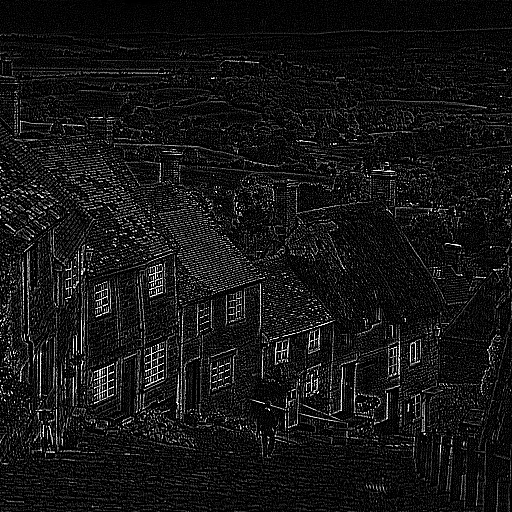
\includegraphics[width=0.9\textwidth]{imagens/city.png}
        \caption{Original: \texttt{city.png}.}
        \label{fig:sharpen:orig}
    \end{subfigure}%
    \begin{subfigure}{0.48\textwidth}
        \centering
        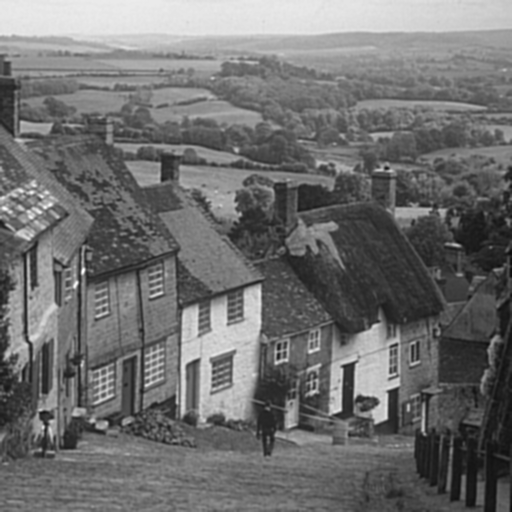
\includegraphics[width=0.9\textwidth]{resultados/city_h2h10.png}
        \caption{Convolução com $h_2$, depois com $h_{10}$.}
        \label{fig:sharpen:combinada}
    \end{subfigure}\\[8pt]
    \begin{subfigure}{0.48\textwidth}
        \centering
        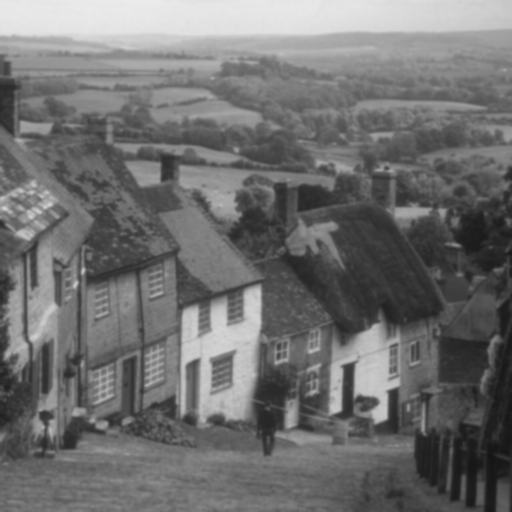
\includegraphics[width=0.9\textwidth]{resultados/city_h2.png}
        \caption{Convolução com $h_2$ (\ref{fig:h2}).}
        \label{fig:sharpen:blur}
    \end{subfigure}%
    \begin{subfigure}{0.48\textwidth}
        \centering
        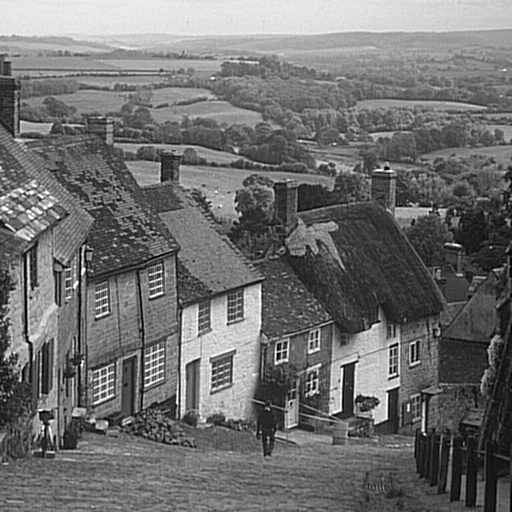
\includegraphics[width=0.9\textwidth]{resultados/city_h10.png}
        \caption{Convolução com $h_{10}$ (\ref{fig:h10}).}
        \label{fig:sharpen:sharpen}
    \end{subfigure}\\[8pt]
    \begin{subfigure}{0.48\textwidth}
        \centering
        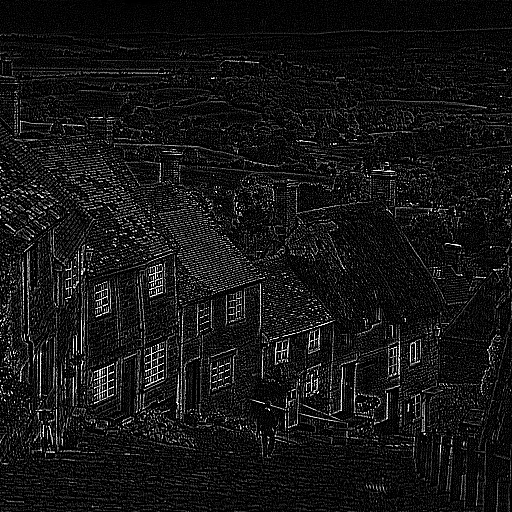
\includegraphics[width=0.9\textwidth]{resultados/city_h5.png}
        \caption{Convolução com $h_5$ (\ref{fig:h5}).}
        \label{fig:sharpen:edge}
    \end{subfigure}%
    \begin{subfigure}{0.48\textwidth}
        \centering
        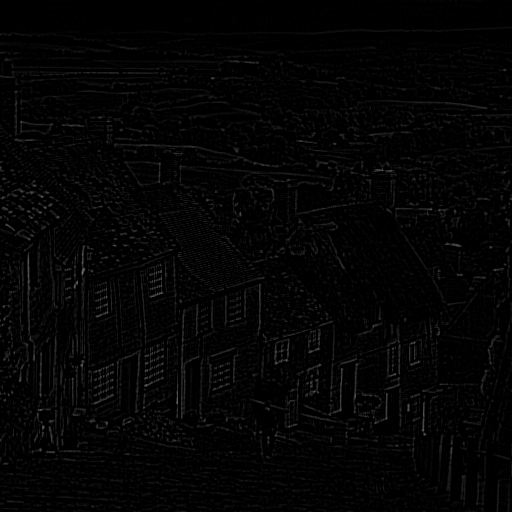
\includegraphics[width=0.9\textwidth]{resultados/city_h10e.png}
        \caption{Convolução com $h_{10}$, removido da original.}
        \label{fig:sharpen:sub}
    \end{subfigure}

    \caption{Filtros de \textit{blur} e de nitidez.}
\end{figure}

Podemos ver nas figuras \ref{fig:sharpen:blur} e \ref{fig:sharpen:sharpen}, comparando com a original (\ref{fig:sharpen:orig}), que o \textit{blur} ($h_2$) reduz a nitidez, enquanto o \textit{sharpen} ($h_{10}$) aumenta. Aplicando o filtro $h_2$ e o $h_{10}$, nessa ordem, resulta na \cref{fig:sharpen:combinada}, que tem nitidez comparável com a original.

A execução desse filtro é pode ser feita com:

\begin{minted}{bash}
    $ python3 main.py imagens/city.png h10
\end{minted}
